% =====================================================================
% Paper A: Multi-Scale Persistent Homology for Competitive Collective
% Systems. arXiv preprint (arxiv.sty). Journal refinement: Journal of
% Quantitative Analysis in Sports (JQAS; De Gruyter dgruyter.sty).
%
% Do not load geometry or fancyhdr here: arxiv.sty already loads both.
% =====================================================================
\documentclass{article}

\usepackage{arxiv}

\usepackage[utf8]{inputenc}
\usepackage[T1]{fontenc}
\usepackage{amsmath,amsfonts,amssymb}
\usepackage{amsthm}
\usepackage{graphicx}
\usepackage{placeins}
\usepackage{flafter}
\usepackage{booktabs}
\usepackage{array}
\usepackage{xurl}
\usepackage{microtype}
\usepackage[numbers,sort&compress]{natbib}
\usepackage{hyperref}

\theoremstyle{plain}
\newtheorem{remark}{Remark}

\title{Multi-Scale Persistent Homology for Competitive Collective Systems}

\author{
 Rowan Brown \\
  Swansea University \\
  \texttt{r.m.brown@swansea.ac.uk}
}

\begin{document}
\maketitle

\begin{abstract}
Competitive collective systems, including sports teams contesting a
pitch, organise at several named levels at once: individuals, small
groups, and a system-wide envelope. Persistent homology records
connected components ($H_0$) and loops ($H_1$) as a distance parameter
grows. On the full point cloud those levels mix in one diagram, so a
change cannot be assigned to a level. This paper asks whether the
homology can be made scale-attributable: each diagram belonging to one
organisational level.
Positions are recorded in metres on a standard football pitch. The
levels are named by how many groups they contain, not by an assumed
length. A cutoff sweep then recovers those distances from the
group-count curve. Hierarchical clustering at those recovered lengths
decomposes the cloud, and persistent homology is computed on the
resulting centroids.
On ten professional matches (broadcast tracking at 10~Hz), three
$H_0$ regimes appear: individual (2.75~m), tactical (11.75~m), and
team (23.0~m). Loops appear at the first two levels, not the third.
Individual-level loops appear in $96.5\%\pm 1.5\%$ of frames (short
bar length in metres); tactical-level loops appear in
$18.8\%\pm 6.5\%$ (longer bar length). Every examined loop is
realised in space, and the two levels carry distinct information.
The same pipeline applies to other bounded competitive systems once
interaction lengths are re-derived.
\end{abstract}

\keywords{Vietoris--Rips filtration \and topological data analysis \and
spatial tracking \and hierarchical clustering \and team sports}

% =======================================================================
\section{Introduction}

\subsection{Background}
\label{sec:background}

Collective systems of agents in space are typically hierarchically
organised. Starling murmurations, fish shoals, and insect swarms, for
example, show individuals, local groups, and a system-wide envelope at
once \citep{sumpter2006}. Understanding how those organisational levels
interact is a standing challenge in applied mathematics, and one that
high-frequency spatial tracking data is increasingly able to inform
\citep{herbertread2011}.

Competitive collective systems are a subset of that class: agents
distributed in a bounded domain, coordinating internally while
responding to an opponent. Examples that share this structure are
autonomous vehicle fleets sharing road space, opposing crowd flows at
transport hubs, predator--prey populations in an ecosystem, and sports
teams contesting pitch or court territory.

Agents in such systems can arrange themselves in ring-like formations
that enclose empty space: milling in a fish school, a vortex in a
swarm, or, in the competitive subset, encirclement of an opponent.
These arrangements are important to identify because enclosure is a
distinct mode of organisation, not a change in density or alignment.
A loop holds a region of space, whether that region is an empty core or
the space denied to an opponent. Conventional geometric summaries,
including convex-hull area, nearest-neighbour distance, and
polarisation, capture dispersion and alignment \citep{sumpter2006} but
do not directly quantify this loop structure.

Persistent homology, a central tool of topological data analysis (TDA),
records connected components ($H_0$) and loops ($H_1$) as a distance
parameter grows
\citep{edelsbrunner2002,edelsbrunner2010,carlsson2009,munch2017,chazal2021}.
A filtration of simplicial complexes indexed by that parameter tracks
the birth and death of those features. Each feature is recorded as a
bar: the interval from the distance at which it appears (birth) to the
distance at which it disappears (death) \citep{ghrist2008}. The length
of the bar distinguishes a stable enclosure from a fleeting coincidence
of positions. The collection of bars is the persistence diagram
\citep{cohensteiner2007}. Efficient computation via the Vietoris--Rips
filtration is due to \citet{bauer2021ripser}; persistence landscapes
provide a functional representation for later statistical analysis
\citep{bubenik2015}.

Persistent homology has recovered cavities in protein atom clouds that
mark flexibility and folding \citep{xia2014}. It has identified
medium-range order in amorphous solids that conventional crystallography
does not resolve \citep{hiraoka2016}. In biological aggregation models
it has shown that distinct swarming organisations appear at different
filtration values \citep{topaz2015}. The same single-parameter
construction, applied directly to a hierarchically organised multi-agent
point cloud, raises the measurement difficulty treated in
Section~\ref{sec:scaleconflation}. This paper asks whether that homology
can be made scale-attributable on a competitive collective system:
each diagram belonging to one organisational level. Opposition couples
successive positions (competitive dependence); that inference problem
is not treated here.

\subsection{The Scale Conflation Problem}
\label{sec:scaleconflation}

A single-parameter Vietoris--Rips filtration on the full point cloud
records features at many filtration values in one persistence diagram.
Bars born at different distances therefore occupy the same object,
whether they arise from local proximity, small-group arrangement, or
system-wide organisation. If that mixing is not recognised, and the
diagram is read as if the cloud had a single organisational level,
features from distinct levels are treated as commensurate. A change in
the diagram then cannot be assigned to a level: it may be a local
rearrangement, a change in group structure, or a change in the system
envelope, and those alternatives are not distinguished. Counts and
persistence summaries inherit the same ambiguity.

Applied studies make that mixing visible without removing it.
Component and loop counts (Betti numbers) from biological aggregation
models, plotted against simulation time and filtration value, show
that distinct swarming organisations appear at different filtration
values \citep{topaz2015}. That display remains one mixed summary. A parallel construction computes
Vietoris--Rips features on multi-agent snapshots and yields a
topological time series at a chosen scale \citep{gu2022}. That series
can detect change points; it does not decompose the cloud by
organisational level.

Responses for the general case exist, but they do not return a
scale-attributable diagram. Multiparameter persistence treats several
scales as simultaneous algebraic parameters \citep{botnan2022}. The
output is a module in several filtration parameters, not a single
persistence diagram that names an organisational level. The
construction is at present computationally feasible only on clouds far
smaller, and sampled far more slowly, than a video-rate cloud of a few
dozen agents. Persistent homology of multiscale clusterings, by
contrast, analyses the hierarchy produced by the clustering itself
\citep{schindler2023}. The output is a topological summary of how
partitions merge as the cutoff varies, not a diagram of loops among
units at one chosen level.

The methods above leave that mixing in place: a bar records when a loop
closes, not which organisational level enclosed it. In a competitive
collective system those levels are named (individual, small group,
envelope), so a superimposed diagram cannot attribute an $H_1$ feature
to a named organisational level, or assign a change in the diagram to
one level rather than another.

\subsection{Contributions}

Section~\ref{sec:scaleconflation} leaves a concrete question: whether
persistent homology can be made scale-attributable on a competitive
collective system. This paper answers that question by changing the
input rather than slicing bars of one diagram.

A cutoff distance $\delta$ groups nearby agents and replaces each group
by its centroid. The reduced cloud then represents one organisational
level, named by how many groups it contains (its cardinality). The
value of $\delta$ is not assumed from the class; it is read from the
group-count curve (Section~\ref{sec:cutoffselection}). Vietoris--Rips
homology is then computed on those centroids. Filtration runs to the diameter of the reduced cloud
(Section~\ref{sec:filtrationextent}). Each $H_1$ bar is realised as a
closed loop in space (Section~\ref{sec:cycles}). Neither clustering
nor that extent rule is algebraically new
\citep{carlsson2010clustering,schindler2023}; the content is that the
combination remains effective on a real, high-frequency, noisy point
cloud.

We test the pipeline on football broadcast tracking: the positions of
all 22 players at $10$~Hz from televised professional matches, as
$(x,y)$ coordinates in metres on a standard pitch model, for ten
A-League matches from the SkillCorner open repository
(Section~\ref{sec:data}). Four questions organise the results, and each
is answered in turn:

\begin{enumerate}
\item\label{q:levels} Can the organisational levels be recovered from
the group-count curve rather than assumed as lengths in metres
(Section~\ref{sec:scaleh0})?
\item\label{q:homology} Does scale-attributable persistent homology
then detect \texorpdfstring{$H_1$}{} loop structure at those levels, is
every feature realised as a loop in space, and is detection robust to
the cutoff and truncation choices
(Sections~\ref{sec:h1detection}--\ref{sec:sensitivity})?
\item\label{q:distinct} Where loops appear at more than one level, do
those levels carry distinct rather than redundant information
(Section~\ref{sec:complementarity})?
\item\label{q:validity} Do the topological features track on-ball match
events, as a construct-validity check only
(Section~\ref{sec:eventcorr})?
\end{enumerate}

Spatial analysis of team sport is surveyed by
\citet{gudmundsson2017} and by \citet{buldu2018} and \citet{grund2012}.
Those methods include pitch-control models and network metrics on
passing and collective structure. They complement the present pipeline
but do not quantify two-dimensional enclosure through persistent
homology. To our knowledge, no prior work combines cutoff-selected
organisational levels with persistent homology for a competitive
collective system, or recovers the resulting regimes on high-frequency
tracking across multiple independent recordings.

% =======================================================================
\section{Methods}

\subsection{Data}
\label{sec:data}

The primary single-match analysis uses SkillCorner open broadcast
tracking data \citep{SkillCorner2024}, match ID 1996435 (Sydney FC
versus Adelaide United, A-League 2024/25). Positions are recorded at
10 frames per second as $(x, y)$ coordinates in metres on a standard
football pitch model. Only frames with complete 22-player coverage are
retained, which yields 43{,}531 frames (approximately 72 minutes at
this sampling rate). The multi-match sample comprises that match and
nine further A-League matches from the same repository. Each match
contributes approximately 39{,}000--49{,}000 complete frames, and the
ten matches together give 436{,}648 frames. SkillCorner match IDs and
fixtures are listed in Supplementary Table~\ref{tab:matches}.

Consecutive complete frames share nearly the same configuration, so
the full stream is not treated as a sequence of independent snapshots.
Connected-component and loop summaries are estimated on a uniform
subsample instead. Write $t$ for the time of a complete frame
in the native stream. The same operational rule is used on every
match: list the complete 22-player frames, set the stride to
$\lfloor N/150\rfloor$, and retain 150 frames. Write $\tilde{t}$ for a
time retained by that rule, and $\tilde{T}$ for the set of such times
on one match, so $|\tilde{T}|=150$. On the primary match
$N = 43{,}531$, so the stride is 290 frames ($\approx 29$~s). Across
ten matches the sampled times give 1{,}500 frames.

This subsample limits temporal pseudo-replication. It does not treat
the competitive-dependence inference problem named in
Section~\ref{sec:background}, and it cannot resolve formation or
dispersion of loops between samples. Event association is a
construct-validity check, not a dynamical model, and it does not use
$\tilde{T}$. Topology for that check is computed on every tenth
complete frame (1~Hz). Supplementary Figure~\ref{fig:acf} records the
autocorrelation of those 1~Hz summaries on the primary match, as a
diagnostic. The figure does not determine the subsample
$\tilde{T}$.

\subsection{Hierarchical clustering}
\label{sec:clustering}

On this corpus the named organisational levels of
Section~\ref{sec:scaleconflation} (individual, small group, envelope)
are instantiated as individual, tactical, and team. Each level is
named by how many groups it contains. The cutoff $\delta$ that
selects it is read from the group-count curve in
Section~\ref{sec:cutoffselection}.

Figure~\ref{fig:pipeline} summarises the pipeline of
Sections~\ref{sec:clustering}--\ref{sec:cycles}. The pipeline is
applied at the sampled times $\tilde{t}\in\tilde{T}$ of
Section~\ref{sec:data}. The input is the point cloud
$P(\tilde{t}) = \{p_1(\tilde{t}), \dots, p_{22}(\tilde{t})\}
\subset \mathbb{R}^2$.

\begin{figure}[t]
\centering
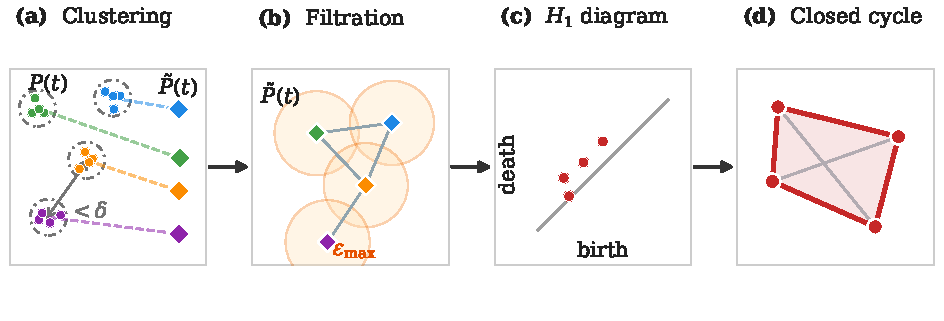
\includegraphics[width=\textwidth]{figures/fig1_pipeline_schematic}
\caption{Analysis pipeline on a bounded domain (schematic geometry on
a football pitch; each panel shows the step and its output).
\textbf{(a)}~Colour-coded local groups in
\texorpdfstring{$P(\tilde{t})$}{}
with dashed \texorpdfstring{$\delta$}{}-disks and a representative
gap \texorpdfstring{$<\delta$}{} (Section~2.2).
\textbf{(b)}--\textbf{(d)}~Vietoris--Rips on the cluster centroids
\texorpdfstring{$\tilde{P}(\tilde{t})$}{} at three increasing
\texorpdfstring{$\varepsilon$}{}, truncated at
\texorpdfstring{$\varepsilon_{\max}$}{}
(equation~\eqref{eq:adaptive}; Section~2.4).
\textbf{(e)}~Finite \texorpdfstring{$H_1$}{} birth--death pairs.
\textbf{(f)}~The same pairs as a barcode.
\textbf{(g)}~Graph-cycle proxy for an \texorpdfstring{$H_1$}{} pair
(Section~2.5). Figure~\ref{fig:cycles} shows the cycle step on real
tracking data.}
\label{fig:pipeline}
\end{figure}

Single-linkage hierarchical clustering is applied at a cutoff
distance $\delta > 0$. It partitions $P(\tilde{t})$ into clusters
$C_1, \dots, C_k$ in which every pair of points is connected by a
chain of pairwise distances not exceeding $\delta$. Each cluster is
replaced by its centroid, giving the reduced point cloud
\[
\tilde{P}(\tilde{t})=\left\{\bar{c}_j : \bar{c}_j=\frac{1}{|C_j|}\sum_{p\in C_j} p,\ j=1,\dots,k\right\},
\]
and persistent homology is then computed on $\tilde{P}(\tilde{t})$
rather than on $P(\tilde{t})$.

Complete-linkage and Ward's method are not used for the headline
analysis. Their effect on $H_1$ counts is examined in
Section~\ref{sec:limitations}. Team identity is withheld as an input,
so the partitions are spatial rather than labelled by side.

\subsection{Cutoff selection}
\label{sec:cutoffselection}

As the cutoff lengthens, nearby agents merge and the mean number of
groups falls. Each organisational level takes its distance from the
point on that curve where the group count named in
Section~\ref{sec:clustering} is reached.

A complete frame has $n=22$ agents. The sweep uses every complete
22-player frame of the ten matches in Supplementary
Table~\ref{tab:matches} (436{,}648 frames). The grid is
$\delta\in[0.25, 40.0]$~m at $0.25$~m steps (160 points). No random
window is drawn, and epoch lengths are not mixed. Clustering is
single-linkage, and team labels are unused.

Let $\overline{H_0}(\delta)$ denote that curve: the mean group count
at cutoff $\delta$, pooled over those frames. Let $P(k\ge 4;\delta)$
be the fraction of frames with at least four groups. The three
inversion rules are then as follows:

\begin{itemize}
\item individual: largest $\delta$ with $\overline{H_0}(\delta)\ge n-3=19$;
\item tactical: $\delta$ minimising
$|\overline{H_0}(\delta)-5|$, among candidates with
$P(k\ge 4;\delta)\ge 0.5$;
\item team: smallest $\delta$ with $\overline{H_0}(\delta)\le 2$.
\end{itemize}
Ties take the smaller $\delta$. The three targets are roster
statements. The individual target $n-3=19$ is a mostly resolved set of
agents. The tactical target $5$, with $k\ge 4$ still common, is a
handful of coordinating groups, enough that a loop remains possible.
The team target $2$ is at most two spatial envelopes.

On this corpus the inversion returns $2.75$~m, $11.75$~m, and
$23.0$~m. Pooled mean group count at those cutoffs is $19.31$,
$5.06$, and $1.98$. Inverting each match separately gives
$2.80\pm 0.20$~m, $11.80\pm 0.35$~m, and $22.98\pm 0.72$~m
(mean $\pm$ s.d.\ across matches). Acceptance requires every match's
mean $\overline{H_0}$ at the pooled cutoff to lie in $[15, 22]$,
$[4, 10]$, and $[1, 2.5]$ respectively. All ten matches lie inside
those bands.

The curve is asymmetric. Nearby agents merge quickly, at about
$1.6$ groups per metre from $\overline{H_0}=19$ to $5$. Larger gaps
then resist merging, at about $0.27$ groups per metre from $5$ to
$2$. The remaining gaps are the large between-group distances. That
flattening is why the team cutoff sits far out at $23.0$~m and still
returns two envelopes, not two teams.

Clustering-quality diagnostics (Calinski--Harabasz, silhouette, and
Shannon entropy of cluster sizes) are recorded on a deterministic
1~Hz subset (every 10th complete frame). Silhouette is omitted when
$k=1$; it is not coded as 0. Those curves are alternatives, not
adopted cutoffs, and are reported in Supplementary
Figure~\ref{fig:diagnostics}. Figure~\ref{fig:cutoff} shows the
estimator and its spatial realisation.
Section~\ref{sec:sensitivity} reports how tactical $H_1$ detection
responds to the cutoff choice.

\begin{figure}[t]
\centering
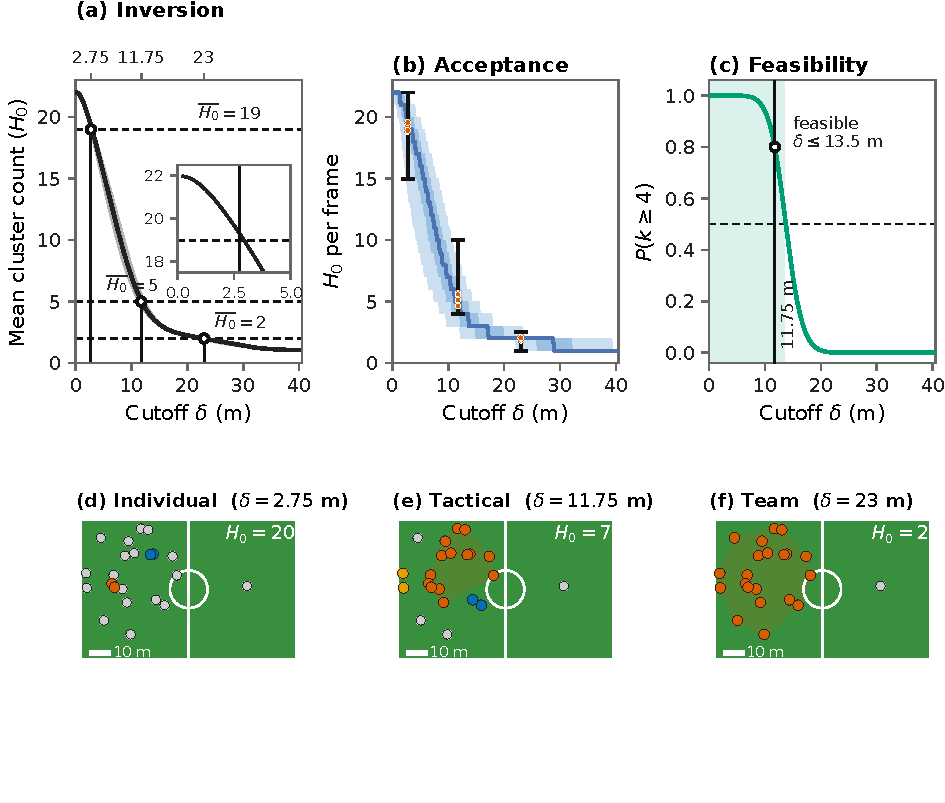
\includegraphics[width=\textwidth]{figures/fig2_cutoff_sweep}
\caption{Cutoff selection from the group-count curve. Sweep on all
complete frames of the ten SkillCorner matches (436{,}648 frames);
not the 150-frame sample \texorpdfstring{$\tilde{T}$}{} of
Section~\ref{sec:data}. Grid
\texorpdfstring{$\delta\in[0.25, 40.0]$}{}~m at $0.25$~m.
\textbf{(a)}~Pooled mean group-count curve
\texorpdfstring{$\overline{H_0}(\delta)$}{} (black) with the ten
per-match curves (grey). Targets are roster statements:
\texorpdfstring{$\overline{H_0}=n-3=19$}{} (most agents resolved),
\texorpdfstring{$\overline{H_0}=5$}{} (a few coordinating groups,
enough that a loop remains possible), and
\texorpdfstring{$\overline{H_0}=2$}{} (two spatial
envelopes, not the two teams, since team labels are unused). Circles
mark the inversion at $2.75$, $11.75$, and $23.0$~m (top axis); the
inset zooms the individual rule.
\textbf{(b)}~Per-frame \texorpdfstring{$H_0$}{} distribution (median,
interquartile band, and 5th--95th centile band). Vertical brackets are
the acceptance intervals \texorpdfstring{$[15,22]$}{},
\texorpdfstring{$[4,10]$}{}, and \texorpdfstring{$[1,2.5]$}{}; orange
dots are the ten per-match means, all inside. Frame-to-frame variance
is why the acceptance intervals, not a single per-frame count, define
the test.
\textbf{(c)}~Feasibility of the tactical rule.
\texorpdfstring{$k$}{} is the number of groups in a frame and
\texorpdfstring{$P(k\ge 4)$}{} the fraction of frames with at least
four; the adopted $11.75$~m sits at \texorpdfstring{$P=0.80$}{}, inside
the feasible region (\texorpdfstring{$\delta\le 13.5$}{}~m).
\textbf{(d--f)}~The same cutoffs on primary-match sample frame~95
(\texorpdfstring{$H_0=20,7,2$}{}; one frame, near the pooled targets
$19$, $5$, $2$). Coloured hulls are multi-player clusters, grey are
singletons; colours distinguish separate topological components in this
frame, not player teams. Each pitch carries a $10$~m scale bar.
Clustering-quality diagnostics are in Supplementary
Figure~\ref{fig:diagnostics} and are not the selector.}
\label{fig:cutoff}
\end{figure}

\subsection{Maximum filtration distance}
\label{sec:adaptivefiltration}

Clustering at cutoff $\delta$ produces a reduced point cloud
$\tilde{P}(\tilde{t})$. Inter-centroid distances on that cloud are typically
larger than $\delta$. A maximum filtration distance
$\varepsilon_{\max}$ fitted to one cutoff can then return no $H_1$ at
another.

The Vietoris--Rips complex itself is not modified. Its parameter is
truncated at
\begin{equation}
\varepsilon_{\max} = \max\Big(P_{75}\{d(\bar c_i,\bar c_j) : i<j\},\; \max(5.0,\,2\delta)\Big).
\label{eq:adaptive}
\end{equation}
Here $P_{75}$ is the 75th percentile of pairwise inter-centroid
distances on $\tilde{P}(\tilde{t})$. The first term tracks the geometry of the
reduced cloud at the current cutoff. The second term is a floor that
prevents a degenerate filtration at small $\delta$. The same floor
keeps the filtration in the inter-cluster distance regime.

$P_{75}$ is a conventional upper-quartile summary.
Section~\ref{sec:sensitivity} reports an ablation across $P_{50}$
through $P_{95}$. Every tested percentile returns identical $H_1$
totals and the same fraction of frames with a loop. The choice is
therefore a reporting convention, not an optimisation.

Persistence diagrams are computed with Ripser via Ripser.py
\citep{bauer2021ripser}, with coefficients in $\mathbb{F}_2$. We report
finite $H_1$ bars. The Results use three summaries of those bars.
\emph{Presence} is the fraction of frames with at least one finite
$H_1$ bar. \emph{Filtration lifetime} $p$ is death minus birth: the
length of a bar, in metres on the Vietoris--Rips parameter.
\emph{Total persistence} is the sum of $p$ over the finite bars in a
frame. It is the Spearman input in
Section~\ref{sec:complementarity}. None of these summaries is a
duration in seconds, and the 150-frame subsample of
Section~\ref{sec:data} does not measure how long a loop lasts on the
clock. The $H_0$ counts reported in
Section~\ref{sec:scaleh0} are read from these diagrams at filtration
zero. We cross-checked all
primary-match diagrams against GUDHI \citep{gudhi2014} and giotto-tda
\citep{tauzin2021}. Birth--death pairs agreed to within numerical
tolerance ($10^{-6}$~m). GUDHI is also used for the bottleneck-distance
and landscape computations reported in
Section~\ref{sec:complementarity}.

\subsection{Closed cycle identification}
\label{sec:cycles}

Each $H_1$ feature corresponds to a 1-cycle in the Vietoris--Rips
complex. A geometric realisation is recovered from the adjacency graph
of edges whose distances fall within the feature's persistence
interval $[\text{birth},\text{death}]$. Closed cycles of at least
three vertices are then enumerated by breadth-first search from each
vertex. If that graph yields no cycle, the search falls back to edges
whose distances lie in
$[\tfrac{1}{2}\text{birth},\,\text{death}]$. Breadth-first
search is used in preference to depth-first search because it
prioritises cycles with fewer vertices. Those cycles correspond to
minimal enclosing arrangements. Among the enumerated cycles, the
representative is the one whose edge distances lie closest to the
midpoint of the persistence interval. This representative is a
geometric proxy for the persistence pair, not a homology generator
extracted from the matrix reduction.

\subsection{Statistical tests}
\label{sec:stats}

$H_1$ detection could reflect the number of centroids rather than
their arrangement. Each frame is therefore compared against a matched
null. For a frame whose clustering yields $k$ centroids, the null
draws $k$ points uniformly from the convex hull of those same
centroids. Group count and spatial envelope are thus held fixed. Only
the arrangement is randomised. The truncation of
equation~\eqref{eq:adaptive} is recomputed on each null cloud.
Nothing else differs between the observed cloud and the null. We use
200 null replicates per frame. The reported statistic is the excess of
observed over null $H_1$ presence, with 95\% confidence intervals from
bootstrap resampling over matches.

Complementarity of the two $H_1$ levels
(Section~\ref{sec:complementarity}) is assessed by two frame-level
tests. The Spearman rank correlation is computed on total $H_1$
persistence: the sum of death minus birth over all finite $H_1$ bars in
a frame. The same correlation is also reported on loop counts, as a
robustness check. Fisher's exact test is computed on the binary
co-occurrence of $H_1$ presence at the two levels. Both statistics
carry 95\% confidence intervals obtained by bootstrap resampling over
matches (1{,}000 resamples), with the match as the resampling unit.
Bottleneck and landscape distances between the two levels' persistence
diagrams are computed using GUDHI, as described in
Section~\ref{sec:adaptivefiltration}.

The construct-validity check in Section~\ref{sec:eventcorr} uses a
Mann--Whitney test of $\Delta$ against zero.
Topology is evaluated on every tenth complete frame (1~Hz), not on
$\tilde{T}$. For each annotated event, $\Delta$ is the change in mean
total persistence from the five 1~Hz frames immediately before the
event to the five immediately after it. That window is five seconds
either side of the event; the event frame itself is excluded.
Event classes are pre-specified, and the $p$-values are nominal.

\subsection{Software and reproducibility}

All analyses were performed in Python~3.11. Persistence diagrams are
computed with Ripser.py~0.6.12 \citep{bauer2021ripser,tralie2018}.
Bottleneck distances and landscape representations use
GUDHI~3.11.0 \citep{gudhi2014}. giotto-tda~0.6.0 \citep{tauzin2021}
provided independent cross-checks. Supporting scientific Python packages
match the pinned \texttt{requirements.txt} accompanying the manuscript:
NumPy~2.0.2, SciPy~1.13.1, pandas~2.3.2, scikit-learn~1.6.1. Analysis
code, pipeline configuration, and pinned dependencies are included with
the manuscript materials. They will be released in a public repository
at arXiv posting (see Data Availability Statement).

% =======================================================================
\section{Results}

\subsection{Connected components (\texorpdfstring{$H_0$}{})}
\label{sec:scaleh0}

Addressing question~\ref{q:levels}, the homology sample confirms the
three organisational levels read from the group-count curve in
Section~\ref{sec:cutoffselection}. Those levels are individual
($\delta = 2.75$~m), tactical ($\delta = 11.75$~m), and team
($\delta = 23.0$~m). Throughout, $H_0$ is the group count: the number
of centroids after clustering. Equivalently, it is $\beta_0$ of the
Vietoris--Rips complex on those centroids at filtration zero.
Primary-match figures come from the uniform 150-frame sample of match
1996435 (Section~\ref{sec:data}). Ten-match aggregates use the same
sampling scheme (1{,}500 frames in total).

At the individual level,
$H_0 = 19.32 \pm 2.34$ (mean $\pm$ s.d.; range 10--22). At the tactical
level, $H_0 = 5.04 \pm 1.69$ (range 2--10). At the
team level, the cloud usually collapses to one or
two groups: mean $1.96 \pm 0.36$. All 22 players lie in a single
group in 8.7\% of frames, split across two in 86.7\%, and across
three in 4.7\%.

The same three-level pattern holds in all ten matches. Grand means are
individual $H_0 = 19.31 \pm 0.31$, tactical $H_0 = 5.09 \pm 0.38$, and
team $H_0 = 1.98 \pm 0.06$ (mean $\pm$ s.d.\ across matches).
Every match stays within the acceptance intervals of
Section~\ref{sec:cutoffselection}: the ten per-match means all fall
inside $[15,22]$, $[4,10]$, and $[1,2.5]$
(Figure~\ref{fig:cutoff}b). Figure~\ref{fig:cutoff} records the sweep
from which those cutoffs were taken. The pooled curve is asymmetric:
about $1.6$ groups merge per metre from the individual to the
tactical level, but only about $0.27$ per metre from the tactical to
the team level, so the two envelopes remain over a wide band
of $\delta$ (Figure~\ref{fig:cutoff}a). The spatial realisation on a
single frame (Figure~\ref{fig:cutoff}d--f) shows the same three
regimes: a mostly resolved set of agents at $2.75$~m, a handful of
coordinating groups at $11.75$~m, and two spatial envelopes at
$23.0$~m, which are topological components rather than the two teams.

\subsection{\texorpdfstring{$H_1$}{} loop detection}
\label{sec:h1detection}

Addressing question~\ref{q:homology}, scale-attributable homology
detects loop structure at two of the three recovered levels. On
the primary match, the pipeline detects 403 $H_1$ loops across 150
uniformly sampled frames (Table~\ref{tab:h1single}). Loops at the
individual level are frequent. They appear in 144 of 150 frames
(96.0\%), at a mean rate of 2.52 per frame, with short filtration
lifetime ($\bar{p}=1.931 \pm 1.735$~m). Loops at the tactical level are
rarer: 23 frames (15.3\%), mean rate 0.17 per frame, with longer
filtration lifetime ($\bar{p}=3.778 \pm 2.723$~m, maximum 10.771~m).
Loops at the team level never occur ($H_1 = 0$ across all 1{,}500
frames in the ten-match sample).

Table~\ref{tab:h1single} collects these statistics in compact form.
$F$ denotes presence: the fraction of frames with at least one loop;
L/f, the mean loop count per frame; $\bar{p}$, mean filtration
lifetime (death minus birth over loops, in metres); and $p_{\max}$,
maximum filtration lifetime.

\begin{table}[h]
\centering
\caption{Single-match \texorpdfstring{$H_1$}{} statistics (primary match, 150 frames).
$\bar{p}$ is the mean of death minus birth over loops, in metres on the
Vietoris--Rips parameter, not a duration in time.}
\label{tab:h1single}
\begin{tabular}{@{}lccccr@{}}
\toprule
Level & Total & $F$ (\%) & L/f & $\bar{p}$ (m) & $p_{\max}$ (m) \\
\midrule
Individual (2.75~m) & 378 & 144/150 (96.0\%) & 2.52 & $1.931\pm1.735$ & 12.991 \\
Tactical (11.75~m)  & 25  & 23/150 (15.3\%)  & 0.17 & $3.778\pm2.723$ & 10.771 \\
Team (23.0~m)       & 0   & 0/150 (0\%)      & N/A  & N/A             & N/A \\
\bottomrule
\end{tabular}
\end{table}

\begin{remark}[Team-level $H_1$ vanishes a priori]
\label{rem:teamnull}
At $\delta = 23.0$~m the 22 players reduce to $k\le 2$ centroids in
93.6\% of complete frames on the ten-match sweep
(Section~\ref{sec:cutoffselection}). A Vietoris--Rips complex on at
most two points cannot carry a non-trivial 1-cycle. Frames with $k=3$
are 6.4\% of that sweep; they are the only team-level configurations
in which a loop is possible. Our headline $H_1$ analysis therefore
runs at two levels (individual and tactical) against the three-level
$H_0$ decomposition above. Team-level loop structure on the typical
envelope would require a different representation (density fields or
Delaunay triangulations, for example).
\end{remark}

The two-level $H_1$ pattern extends to all ten matches (1{,}500
uniformly sampled frames; Table~\ref{tab:h1multi}). Individual-level
presence is $96.5\%\pm1.5\%$ (95\% CI $95.6$--$97.3\%$), between 94.7\%
and 98.7\% in every match. Tactical presence is $18.8\%\pm6.5\%$ (95\%
CI $15.2$--$22.7\%$), ranging from 11.3\% to 31.3\% across matches. The
primary match (15.3\% tactical) sits within one standard deviation of
the ten-match mean. That match was chosen for broadcast quality and
event annotation, not for its tactical $H_1$ rate.
Conditional mean filtration lifetime on the ten-match sample is
$1.886$~m at the individual level and $3.411$~m at the tactical level,
the same ordering as Table~\ref{tab:h1single}.

\begin{table}[h]
\centering
\caption{Multi-match \texorpdfstring{$H_1$}{} statistics (10 matches).
Presence = mean \texorpdfstring{$\pm$}{} s.d.\ across matches; 95\%
bootstrap CIs from 1{,}000 resamples over matches.
$\bar{p}$ is mean filtration lifetime over loops
(\texorpdfstring{$\sum p / \sum H_1$}{}), not the per-frame average
that includes zeros. The s.d.\ column is the standard deviation of the
ten per-match conditional means.}
\label{tab:h1multi}
\begin{tabular}{@{}lccccr@{}}
\toprule
Level & Total & Presence (\%) & 95\% CI & $\bar{p}$ (m) & s.d. \\
\midrule
Individual & 4{,}039 & $96.5\%\pm1.5\%$ & $95.6$--$97.3\%$ & 1.886 & 0.145 \\
Tactical   & 306     & $18.8\%\pm6.5\%$ & $15.2$--$22.7\%$ & 3.411 & 0.419 \\
Team       & 0       & $0.0\%\pm0.0\%$  & N/A              & N/A   & N/A \\
\bottomrule
\end{tabular}
\end{table}

The tactical level sits close to a group-count floor. In the
ten-match sample, 40.6\% of frames have four or fewer tactical groups.
None of those frames carries a loop.

Presence alone cannot separate arrangement from group count. The
matched null of Section~\ref{sec:stats} holds the group count and the
spatial envelope fixed, and randomises only the arrangement inside
that envelope.

Table~\ref{tab:null} gives the comparison. Tactical presence is
18.8\%, against a null rate of 9.1\%, an excess of $+9.7$ percentage
points. Table~\ref{tab:nullk} splits the same comparison by group
count. Presence is zero for $k\le 4$. It then rises from 9.3\% at
$k=5$ to 67.0\% at $k=8$, and remains above the null at every such
$k$.

At the individual level the null rate is already 91.4\%. Twenty points
in a bounded region almost always close a cycle, so the observed
excess is modest ($+5.1$ percentage points).

\begin{table}[h]
\centering
\caption{\texorpdfstring{$H_1$}{} presence against a group-count- and envelope-matched null (10 matches, 1{,}500 frames, 200 null replicates per frame). Excess is in percentage points, with 95\% bootstrap CIs over matches.}
\label{tab:null}
\begin{tabular}{@{}lcccc@{}}
\toprule
Level & Observed & Null & Excess & 95\% CI \\
\midrule
Individual & 96.5\% & 91.4\% & $+5.1$ & $[+3.9, +6.1]$ \\
Tactical   & 18.8\% & 9.1\%  & $+9.7$ & $[+7.3, +12.2]$ \\
\bottomrule
\end{tabular}
\end{table}

\begin{table}[h]
\centering
\caption{Tactical-level \texorpdfstring{$H_1$}{} presence by group count \texorpdfstring{$k$}{}, against the matched null of Table~\ref{tab:null} (10 matches, 1{,}500 frames).}
\label{tab:nullk}
\begin{tabular}{@{}rcccc@{}}
\toprule
$k$ & Frames & Observed & Null & Excess \\
\midrule
$\le 4$ & 609 & $0.0\%$ & $0.4\%$ & $-0.4$ \\
5 & 344 & $9.3\%$ & $4.1\%$ & $+5.2$ \\
6 & 252 & $26.6\%$ & $12.0\%$ & $+14.5$ \\
7 & 149 & $51.0\%$ & $21.7\%$ & $+29.3$ \\
8 & 94 & $67.0\%$ & $33.4\%$ & $+33.6$ \\
$\ge 9$ & 52 & $84.6\%$ & $49.0\%$ & $+35.6$ \\
\bottomrule
\end{tabular}
\end{table}

\subsection{Closed cycle structures}
\label{sec:cyclegeometry}

All 403 primary-match $H_1$ features receive a geometric realisation
via closed-cycle identification. The representative is the graph-cycle
proxy of Section~\ref{sec:cycles}, not a generator from the reduction
matrix. Cycles at the individual level form short rings of centroids
(typically three to six vertices in the examples we inspected). Tactical
cycles are similarly small (often four or five vertices) but span larger
gaps and have larger filtration lifetime. Figure~\ref{fig:cycles} shows the same sample
frame at both levels, with the cutoff and the filtration drawn as
separate panels (sample frame~95). The left column is the vertex set
after clustering. The right column is the
\texorpdfstring{$H_1$}{} cycle of largest $p$ on that set.
At \texorpdfstring{$\delta=2.75$}{}~m the vertices are four nearby
players and the cycle edges are $17.8$--$19.2$~m
(\texorpdfstring{$p=6.540$}{}~m).
At \texorpdfstring{$\delta=11.75$}{}~m the vertices are four groups,
one of them a $14$-player single-linkage cluster, and the cycle edges
are $21.1$--$28.8$~m (\texorpdfstring{$p=9.942$}{}~m).
The two cycles are not the same bar at two resolutions.
Figure~\ref{fig:h1bars} shows those bars on the persistence diagram,
together with every finite $H_1$ bar on the primary match.
The bars of largest $p$ in Table~\ref{tab:h1single} are not used for
the figure: the individual-level bar of largest $p$ (frame~141) is a
near-collinear sliver.

\begin{figure}[tp]
\centering
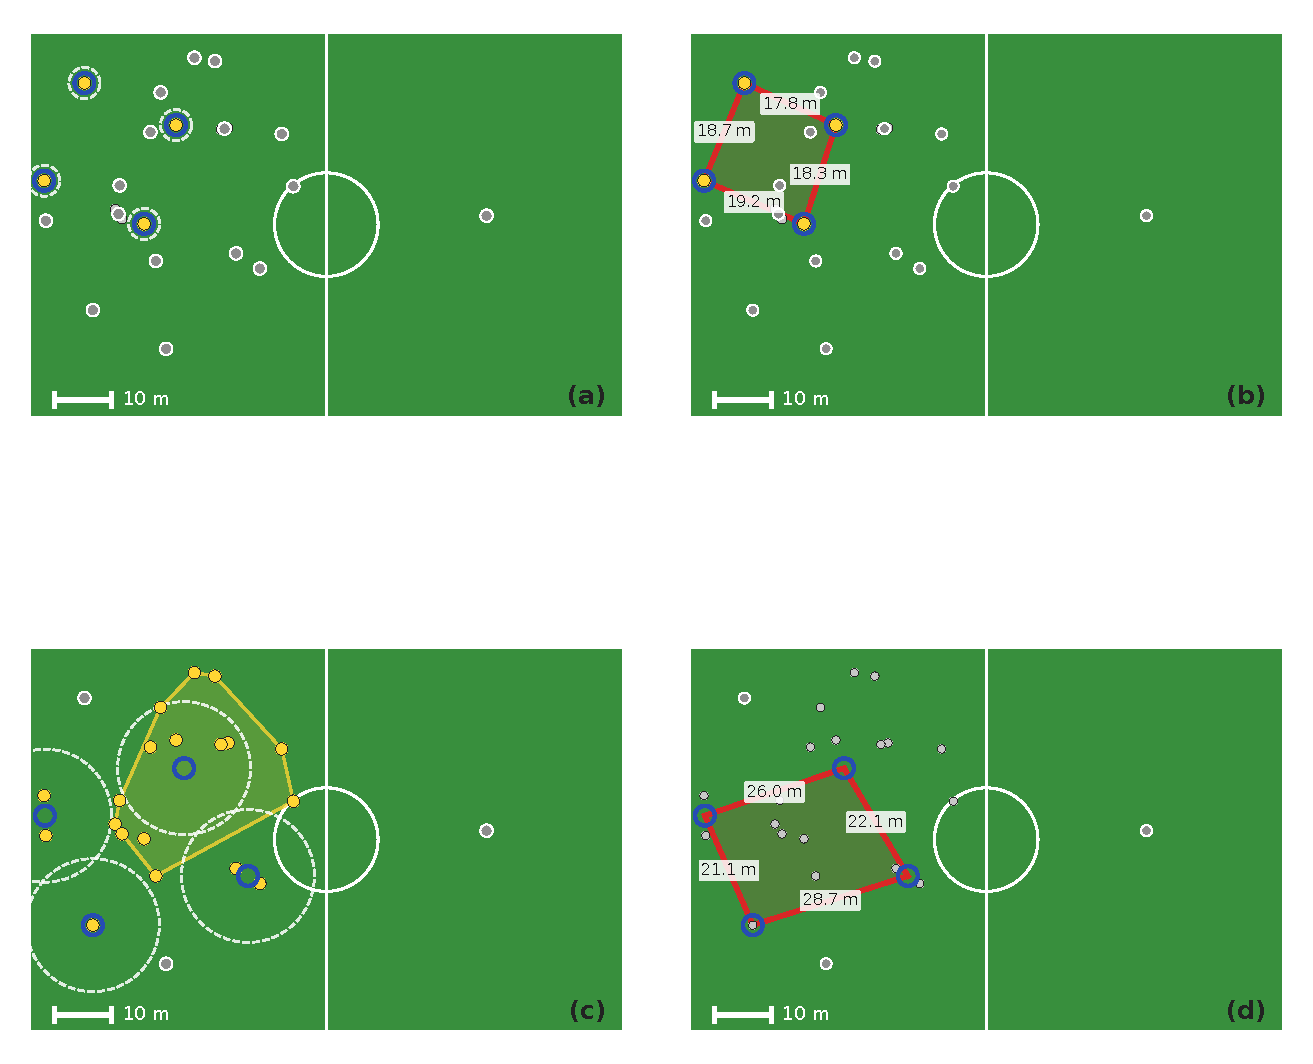
\includegraphics[width=\textwidth,keepaspectratio]{figures/fig3_cycle_geometry}
\caption{Cutoff versus filtration on one sample frame of SkillCorner
match 1996435 (sample frame~95). Left: vertex set after clustering at
\texorpdfstring{$\delta$}{}. Gold markers belong to this row's cycle
clusters; the hull in (c) is the 14-player single-linkage cluster;
dashed circles have radius \texorpdfstring{$\delta$}{} on the cycle
vertices only. Right: \texorpdfstring{$H_1$}{} representative of
largest \texorpdfstring{$p$}{} on those vertices
(\texorpdfstring{$p=6.540$}{}~m and
\texorpdfstring{$p=9.942$}{}~m). Cycle edges are filtration
distances (\texorpdfstring{$17.8$--$19.2$}{}~m in (b);
\texorpdfstring{$21.1$--$28.8$}{}~m in (d)), not the cutoff.
Panel (d) draws centroids, not the absorbed players.
Compact four-cycles at both levels, not the bar of largest
\texorpdfstring{$p$}{} on the match.
A 10~m scale bar is shown on each panel. Uniform sample,
\texorpdfstring{$n=150$}{} frames, every 290th complete frame (the
same rule as the ten-match analysis).}
\label{fig:cycles}
\end{figure}

\begin{figure}[tp]
\centering
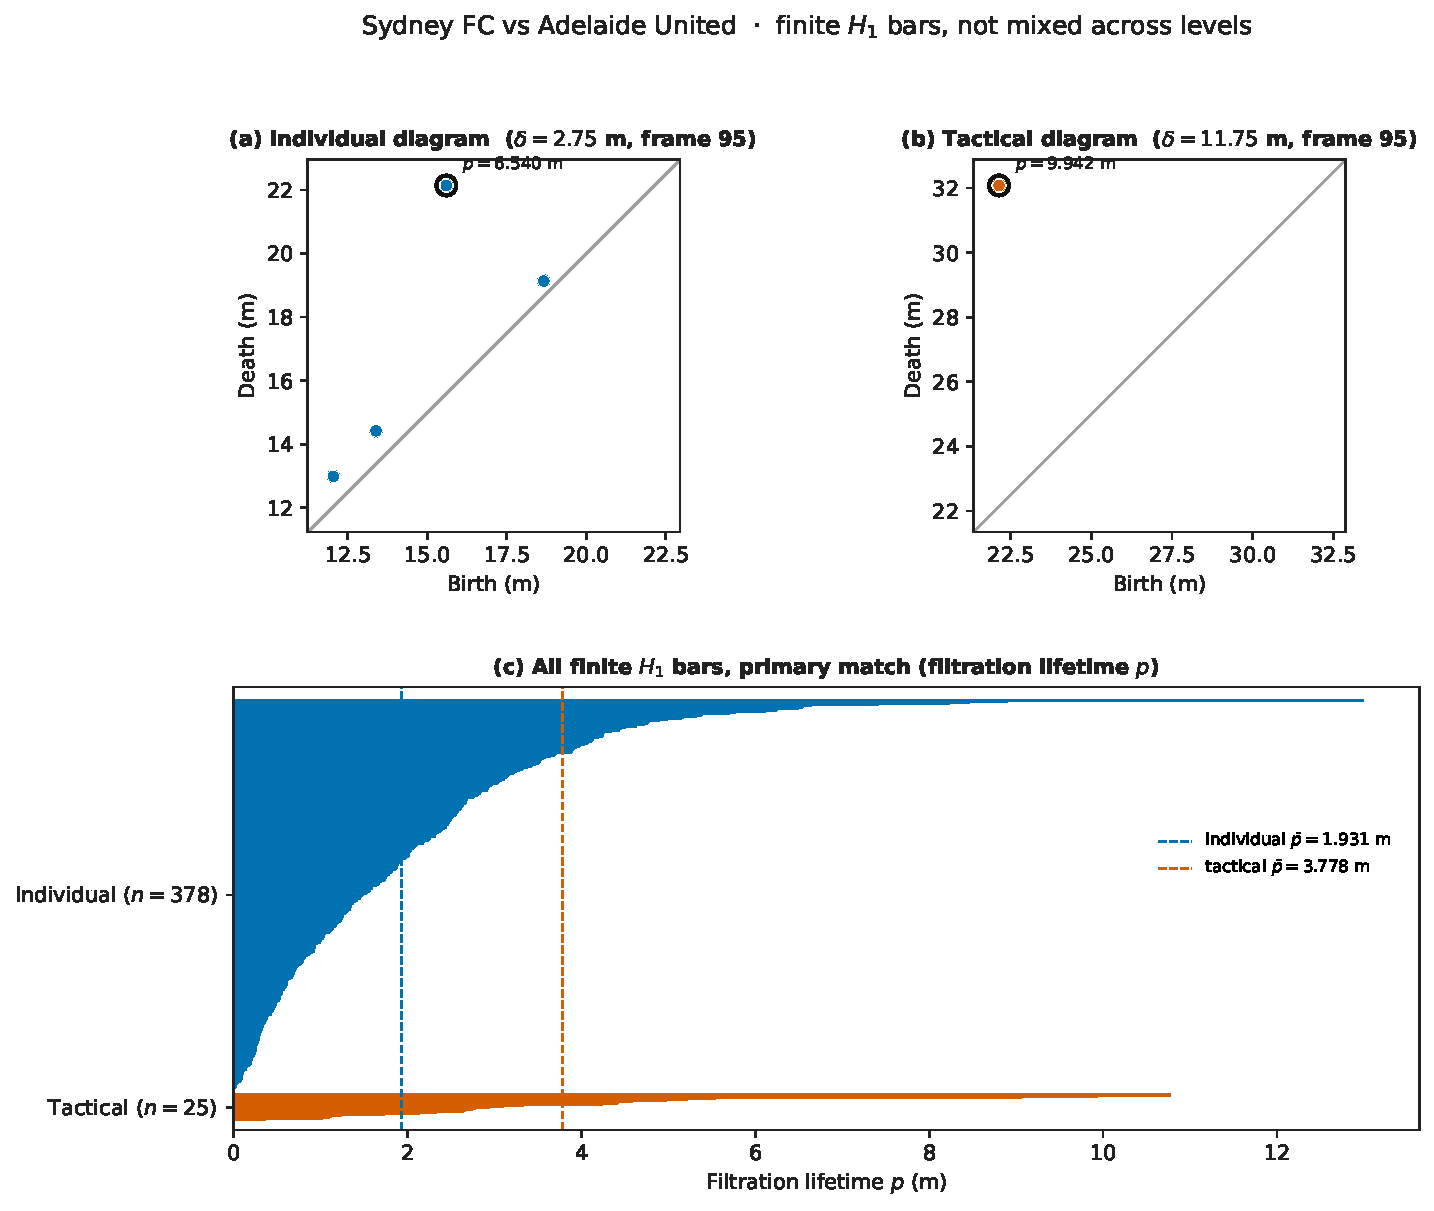
\includegraphics[width=\textwidth,keepaspectratio]{figures/fig4_h1_diagrams}
\caption{Finite \texorpdfstring{$H_1$}{} bars at two organisational
levels on the primary match (uniform 150-frame sample).
\textbf{(a)}~Individual and \textbf{(b)}~tactical persistence diagrams
for sample frame~95, the same frame as Figure~\ref{fig:cycles}.
The marked pair is the bar of largest \texorpdfstring{$p$}{} on that frame
(\texorpdfstring{$p=6.540$}{}~m and
\texorpdfstring{$p=9.942$}{}~m), whose geometric representative appears
in Figure~\ref{fig:cycles}.
\textbf{(c)}~Every finite bar on the primary match, one track per
organisational level (378 individual, 25 tactical).
The dashed ticks are Table~\ref{tab:h1single}'s $\bar{p}$: the mean of
these bar lengths (death minus birth, in metres of the Vietoris--Rips
parameter \texorpdfstring{$\varepsilon$}{}, not seconds).
The two levels are not superimposed: that would recreate the mixing of
Section~\ref{sec:scaleconflation}.
The individual-level bar of largest \texorpdfstring{$p$}{} in
Table~\ref{tab:h1single} (frame~141) is a near-collinear sliver and is
not the cycle shown in Figure~\ref{fig:cycles}.}
\label{fig:h1bars}
\end{figure}

\subsection{Sensitivity analysis}
\label{sec:sensitivity}

Detection is not confined to the adopted cutoff or to a single
truncation percentile. Tactical $H_1$ counts fall monotonically
as the cutoff widens. On the
primary match's 150 frames, sweeping $\delta\in[6,16]$~m gives 275
loops (87.3\% of frames) at $\delta=6$~m and none at $\delta=16$~m.
The operative range is $[6,14]$~m (Table~\ref{tab:sensitivity}). The
adopted cutoff $\delta=11.75$~m lies at the conservative end of that
range (15.3\% frame presence).

\begin{table}[h]
\centering
\caption{Tactical-level cutoff sensitivity (150 frames, primary match).}
\label{tab:sensitivity}
\begin{tabular}{@{}lccc@{}}
\toprule
$\delta$ (m) & Total $H_1$ & Frame presence & Mean $H_0$ \\
\midrule
6  & 275 & 87.3\% & 13.4 \\
8  & 162 & 68.0\% & 9.8 \\
10 & 78  & 42.7\% & 7.0 \\
11.75 & 25 & 15.3\% & 5.0 \\
12 & 21  & 12.7\% & 4.8 \\
14 & 5   & 3.3\%  & 3.5 \\
16 & 0   & 0.0\%  & 2.8 \\
\bottomrule
\end{tabular}
\end{table}

The truncation in equation~\eqref{eq:adaptive} is likewise stable. At
$\delta=11.75$~m, every percentile from $P_{50}$ to $P_{95}$ yields the
same 25 loops and 15.3\% frame presence, even though mean
$\varepsilon_{\max}$ spans 37.6--65.3~m
(Table~\ref{tab:percentile}).

\begin{table}[h]
\centering
\caption{Filtration-percentile ablation, \texorpdfstring{$\delta=11.75$}{}~m.}
\label{tab:percentile}
\begin{tabular}{@{}lccc@{}}
\toprule
Percentile & Total $H_1$ & Frame presence & Mean $\varepsilon_{\max}$ (m) \\
\midrule
$P_{50}$ & 25 & 15.3\% & 37.6 \\
$P_{60}$ & 25 & 15.3\% & 41.8 \\
$P_{75}$ & 25 & 15.3\% & 49.6 \\
$P_{90}$ & 25 & 15.3\% & 60.0 \\
$P_{95}$ & 25 & 15.3\% & 65.3 \\
\bottomrule
\end{tabular}
\end{table}

\subsection{Complementarity of the two \texorpdfstring{$H_1$}{} levels}
\label{sec:complementarity}

The two $H_1$ levels carry distinct rather than redundant
information.
Over 1{,}500 uniformly sampled frames, total individual and tactical
$H_1$ persistence correlate weakly (Spearman $\rho=0.234$, $p<0.001$;
95\% bootstrap CI $[0.181, 0.276]$). The same holds for loop counts
($\rho=0.205$, $p<0.001$). The finding does not depend on whether the
comparison uses total persistence or loop counts.

Co-occurrence exceeds chance (Fisher odds ratio 6.12, $p=0.002$;
bootstrap CI $[2.32, 16.33]$). Table~\ref{tab:fisher} shows the
asymmetry: 1{,}167 frames carry individual loops without a tactical
partner, and only two frames do the reverse. Weak rank correlation
remains the main evidence for complementarity. Joint presence need not
mean the two levels measure the same structure.

\begin{table}[h]
\centering
\caption{Frame counts of \texorpdfstring{$H_1$}{} presence at the two levels (1{,}500 frames).}
\label{tab:fisher}
\begin{tabular}{@{}lcc@{}}
\toprule
 & Tactical $H_1$ present & Tactical $H_1$ absent \\
\midrule
Individual $H_1$ present & 280 & 1{,}167 \\
Individual $H_1$ absent  & 2   & 51 \\
\bottomrule
\end{tabular}
\end{table}

Bottleneck distance between the two levels'
diagrams has median 1.456~m and 95th-percentile tail 3.556~m. That is
on the order of typical tactical filtration lifetime on the primary
match (3.778~m mean bar length where loops appear;
Table~\ref{tab:h1single}). Landscape $L^2$ distance has median 5.477.
The levels differ by roughly as much as their features are large, not
by a small perturbation of one shared pattern.

\subsection{Event correlation}
\label{sec:eventcorr}

Addressing question~\ref{q:validity}, total persistence moves with
on-ball events. The comparison is a construct-validity check against
measurement noise. It uses 103{,}856 SkillCorner event--topology pairs
from the ten matches.

For each event, $\Delta$ is the change in mean total persistence from
the five 1~Hz frames before the event to the five after it
(Section~\ref{sec:stats}). At the individual level, an on-ball
engagement is followed by a drop. The mean change is
$\Delta=-0.253$~m ($n=8{,}927$, Mann--Whitney $p<10^{-13}$).
Build-up is followed by a rise. The mean change is
$\Delta=+0.700$~m ($n=618$, $p<10^{-6}$). At the tactical level,
engagements are again followed by a drop and build-up by a rise.

The event classes were specified in advance, and the $p$-values are
nominal. Multiple-testing control and a football reading of these
shifts belong to a companion manuscript.

% =======================================================================
\section{Discussion}

\subsection{Recovered organisational levels}
\label{sec:disc-levels}

The three $H_0$ regimes
(individual, tactical, and team) are the named group-count targets of
Section~\ref{sec:cutoffselection}, read from the pooled group-count
curve on every complete frame of the
ten matches (Figure~\ref{fig:cutoff}). Those regimes remain over a
range of $\delta$ rather than appearing only at the adopted cutoffs.
The metre values are specific to this corpus. Another domain still
requires the interaction lengths to be re-derived.

The tactical distance is the point on that curve where the mean group
count lies nearest five, and where frames with at least four groups
are still common (Figure~\ref{fig:cutoff}c). On the 1~Hz diagnostic
subset, the silhouette score has one interior local maximum, at
$7.0$~m. That distance is a small-group alternative. Once frames that
have collapsed to a single group are omitted, the score rises again
through the two-envelope regime (Supplementary
Figure~\ref{fig:diagnostics}). We record that curve and keep the
group-count cutoff.

\subsection{Two \texorpdfstring{$H_1$}{} regimes}
\label{sec:disc-homology}

Scale-attributable homology
detects loops at two of the three recovered levels. Individual-level
loops are frequent; tactical-level loops are rarer and have longer
filtration lifetime (Tables~\ref{tab:h1single}--\ref{tab:h1multi};
Figure~\ref{fig:h1bars}). Filtration lifetime is the bar length
(death minus birth, in metres). It is not how long a loop lasts on the
clock. The 150-frame subsample does not resolve formation or
dispersion of loops between samples (Section~\ref{sec:data}).

Every examined $H_1$ feature is realised as a loop in space
(Figure~\ref{fig:cycles}). Detection is not confined to the adopted
cutoff (Section~\ref{sec:sensitivity}). Tactical $H_1$ is detected on the
band $[6,14]$~m, not only at an isolated optimum.

The pipeline therefore reports three $H_0$ regimes and two $H_1$
regimes. At the team level the reduced cloud almost never has enough
groups to close a loop (Remark~\ref{rem:teamnull}). Recovering
team-level loop structure on the typical envelope would require a
different representation, such as spatial density fields or Delaunay
triangulations. Linkage choice changes tactical $H_1$ counts by nearly
an order of magnitude; that caveat is taken up in
Section~\ref{sec:limitations}.

\subsection{Distinct structure at two levels}
\label{sec:disc-distinct}

The two $H_1$ levels carry distinct rather than redundant
information. They are not measuring the same structure at different
resolutions. If the tactical signal were a coarsened version of the
individual signal, the two would co-occur far more consistently than
Table~\ref{tab:fisher} shows. The bottleneck and landscape distances
would also be small relative to each level's own filtration lifetimes
(Section~\ref{sec:complementarity}).
Clustering before persistent homology is therefore not a convenience
for separating noise. It produces two informationally distinct
objects.

\subsection{Construct validity}
\label{sec:disc-validity}

Total persistence moves with on-ball events
(Section~\ref{sec:eventcorr}). At the individual level, an engagement
is followed by a mean drop of $0.253$~m, and build-up by a mean rise
of $0.700$~m. At the tactical level the two classes move in the same
direction. That movement is the construct-validity check against
measurement noise. Multiple-testing control and a football reading of
the shifts belong to a companion manuscript (Paper~B).

\subsection{Limitations}
\label{sec:limitations}

Linkage selection is a substantive methodological choice for the
composed map (cluster at $\delta$, then Vietoris--Rips on centroids).
Across a 600-frame, four-match comparison sample, single-linkage
detects 106 tactical-level $H_1$ loops. Complete-linkage detects 802.
Ward's method detects 822. That is a difference of almost an order of
magnitude. Point-cloud stability theorems do not bound this map when
single-linkage jumps at merge events; characterising diagram stability
under clustering is an open problem we defer to follow-on work. The gap is large enough to change which scientific picture
the data support, not merely the precision of one estimate. We retain
single-linkage because its definition is the most natural reading of
spatial proximity. It is also robust against over-partitioning artefacts.

A more principled selection criterion would come from the dynamical
system itself, rather than from clustering-quality metrics alone. One
candidate is the linkage under which a governing equation for a
persistence functional admits the sparsest representation, in the
sense of sparse identification of nonlinear dynamics. The functional
would be the landscape $L^2$ norm or the tactical $H_1$
total-persistence sequence. Operationalising this would require three
things. First, choose the dynamical state. Second, defend the sparsity
of the recovered library against the Akaike information criterion
(AIC), the Bayesian information criterion (BIC), or cross-validation
baselines. Third, confirm that the resulting persistence sequence is
genuinely lower-dimensional under the selected linkage. We defer this
to the forthcoming full-season work. A population-sized sample of
match sequences is what makes the sparsity comparison meaningful.

A landscape-path stability criterion (minimise variation of the
persistence landscape under small perturbations of $\delta$) remains a
future estimator of the tactical cutoff. It is computable with the
landscape infrastructure of Section~\ref{sec:complementarity}. We
defer it to the persistence-landscape companion work.
Section~\ref{sec:sensitivity} reports the $[6,14]$~m tactical
$H_1$ band as an empirical property around the adopted $11.75$~m.

All data analysed here are broadcast-derived tracking at 10~Hz.
Broadcast tracking typically offers lower spatial precision than
higher-frequency optical systems. That may affect the magnitude of
filtration lifetimes reported. The structural findings (the three
$H_0$ regimes, the $H_1$ presence rates, and the sensitivity profiles)
depend on relative rather than absolute spatial precision. They are
therefore expected to be robust across tracking technologies. A
direct comparison of filtration lifetimes against optical tracking
data remains for future work.

\subsection{Outlook}

Two extensions are in progress. The ten-match evidence base is being scaled
to a full season of Championship matches. That sample will
characterise population-level distributions of $H_0$ and $H_1$
counts, filtration lifetimes, and landscape norms, and will test
whether matches carry a stable tactical signature at population
scale. It is also
the setting in which the linkage criterion proposed above becomes
evaluable. Recovering a sparse governing equation for a persistence
functional requires the population-sized sample of match sequences
that a single season provides. Separately, persistence landscape
dynamics are being developed to treat each match as a path through
landscape space. That is the setting in which the landscape-stability
cutoff criterion can itself be evaluated. Its resampling unit is the
match-level landscape, not the per-frame summary used here.

% =======================================================================
\section{Conclusion}

On ten professional football matches, clustering at recovered
interaction lengths and a truncation of the Vietoris--Rips parameter
produced three $H_0$ regimes and two $H_1$ regimes. Every
examined $H_1$ feature is realised as a loop in space. The two
$H_1$ levels carry distinct rather than redundant information.
Those findings answer whether persistent homology can be made
scale-attributable on a competitive collective system: each diagram
belonging to one organisational level. Football was the measurement
setting. The same pipeline applies to other bounded competitive
systems once interaction lengths are re-derived.

% =======================================================================
\section*{Declarations}

\subsection*{Competing Interests}
The authors have no competing interests to declare.

\subsection*{Acknowledgements}
The authors thank SkillCorner for use of the open broadcast tracking
dataset.

\subsection*{Funding}
This research received no specific grant from any funding agency in the
public, commercial, or not-for-profit sectors; it was conceived and
conducted independently by the authors.

\subsection*{Data Availability Statement}
Positional tracking data were provided by SkillCorner under an open-data
licence (\url{https://github.com/SkillCorner/opendata}). Analysis code,
pipeline configuration, pinned \texttt{requirements.txt}, and the result
files used for the figures and tables in this paper are included with
the manuscript materials and will be released in a dedicated public
repository at arXiv posting, deposited in the Swansea University Zenodo community.

\subsection*{Use of Large Language Models}
% NOTE: Springer's policy requires disclosure when AI tools are used
% beyond copy-editing. Review and finalise this statement before submission.
Large language model (LLM) tools were used during the preparation of this
manuscript to assist with prose structuring and copy-editing. All
scientific content, analyses, interpretations, and conclusions are the
sole responsibility of the authors. No LLM tool was used to generate
novel scientific claims or to conduct or interpret statistical analyses.

\section*{Supplementary note: temporal autocorrelation}
\label{sec:acf}

Headline $H_0$ and $H_1$ tables use the uniform 150-frame rule of
Section~\ref{sec:data}. Supplementary Figure~\ref{fig:acf} is a
diagnostic on the primary match at 1~Hz; it does not choose the stride.
Generate with \texttt{pipeline/steps/09\_acf\_supplement.py}.

\IfFileExists{figures/figS1_acf.pdf}{%
\begin{figure}[h]
\centering
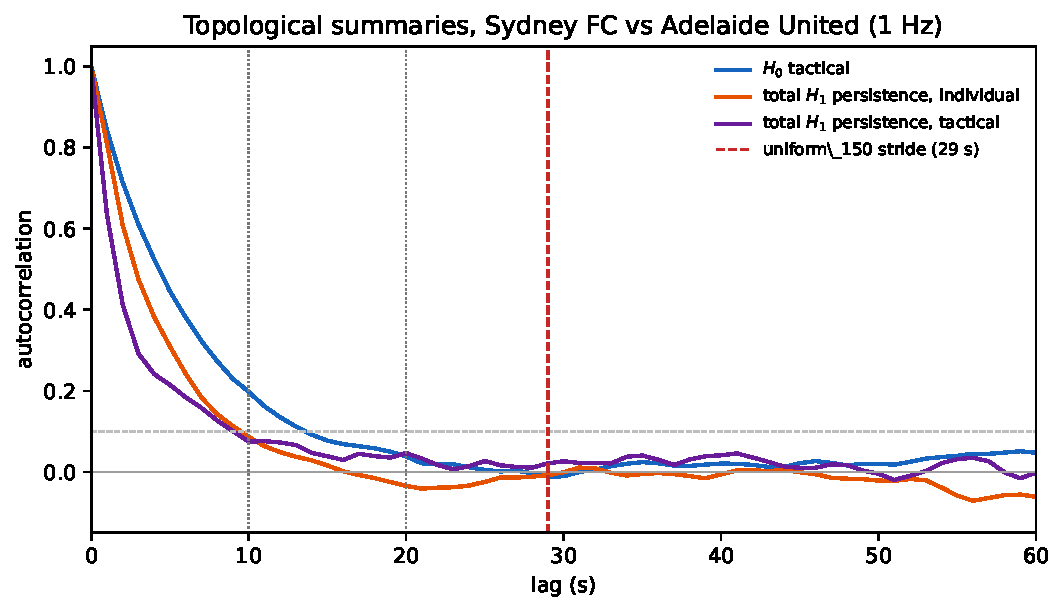
\includegraphics[width=0.85\textwidth]{figures/figS1_acf}
\caption{Autocorrelation of frame-level topological summaries on
SkillCorner match 1996435 at 1~Hz. Series: tactical
\texorpdfstring{$H_0$}{}, and total \texorpdfstring{$H_1$}{}
persistence at the individual and tactical levels. The dashed red line
is the uniform-150 stride.}
\label{fig:acf}
\end{figure}
}{%
\par\textit{Supplementary Figure~S1 is not yet generated. Run
\texttt{09\_acf\_supplement.py} once SkillCorner open data are available.}
\label{fig:acf}
}

\section*{Supplementary note: clustering-quality diagnostics}
\label{sec:diagnostics}

The cutoffs in Figure~\ref{fig:cutoff} are read from the group-count
curve, not from a clustering-quality score. For completeness we
record three standard diagnostics on a deterministic 1~Hz subset
(every 10th complete frame): the Calinski--Harabasz index, the mean
silhouette score, and the Shannon entropy of cluster sizes
(information-content). Silhouette is undefined when a frame collapses
to a single cluster ($k=1$); those frames are omitted rather than
coded as 0. None of these curves selects the adopted cutoffs.

The silhouette rises again beyond the tactical level. This is an
artefact of the shrinking $k\ge 2$ subsample: as $\delta$ grows, only
frames that still hold two or more widely separated envelopes
contribute, and such configurations are trivially well separated. The
only interior silhouette local maximum is at $7.0$~m, a small-group
alternative that we report but do not adopt.

\IfFileExists{figures/figS2_cutoff_diagnostics.pdf}{%
\begin{figure}[h]
\centering
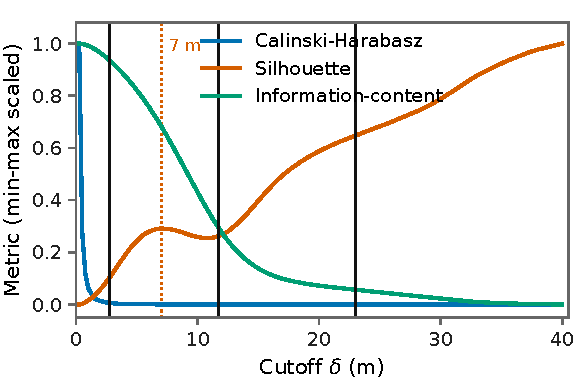
\includegraphics[width=0.62\textwidth]{figures/figS2_cutoff_diagnostics}
\caption{Clustering-quality diagnostics on the 1~Hz subset, each
min-max scaled to \texorpdfstring{$[0,1]$}{} for display: the
Calinski--Harabasz index, the mean silhouette score, and
information-content. Solid vertical lines mark the adopted cutoffs
($2.75$, $11.75$, $23.0$~m); the dotted line marks the interior
silhouette local maximum ($7.0$~m). The silhouette rise at large
\texorpdfstring{$\delta$}{} reflects the shrinking
\texorpdfstring{$k\ge 2$}{} subsample, not a better partition. These
quality metrics are diagnostics, not the selector.}
\label{fig:diagnostics}
\end{figure}
}{%
\par\textit{Supplementary Figure~S2 is not yet generated. Run
\texttt{pipeline/steps/10\_cutoff\_sweep\_figure.py} once the
diagnostics subset has been written.}
\label{fig:diagnostics}
}

\section*{Supplementary Table S1. SkillCorner match identifiers}

Ten A-League matches from the SkillCorner open repository. Home and
away names are those recorded in the tracking files. The primary match
is used for single-match $H_1$ tables, cycle geometry, and
Figure~\ref{fig:acf}.

\begin{table}[h]
\centering
\caption{SkillCorner match identifiers.}
\label{tab:matches}
\begin{tabular}{@{}llll@{}}
\toprule
SkillCorner ID & Home & Away & Role \\
\midrule
1886347 & Auckland FC & Newcastle & multi-match \\
1899585 & Auckland FC & Wellington P FC & multi-match \\
1925299 & Brisbane FC & Perth Glory & multi-match \\
1953632 & CC Mariners & Melbourne City & multi-match \\
1996435 & Sydney FC & Adelaide United & primary \\
2006229 & Melbourne City & Macarthur FC & multi-match \\
2011166 & Wellington P FC & Melbourne V FC & multi-match \\
2013725 & Western United & Sydney FC & multi-match \\
2015213 & Western United & Auckland FC & multi-match \\
2017461 & Melbourne V FC & Auckland FC & multi-match \\
\bottomrule
\end{tabular}
\end{table}


\FloatBarrier
\bibliographystyle{unsrtnat}
\bibliography{references}

\end{document}
